%!TEX root = thesis.tex
\chapter{Data, Preprocessing and Features}\label{ch:preprocessing}

\begin{wrapfigure}{r}{7cm}
  \vspace{-35pt}
  \begin{center}
    \newcommand*{\xMin}{0}%
    \newcommand*{\xMax}{6}%
    \newcommand*{\yMin}{0}%
    \newcommand*{\yMax}{6}%
    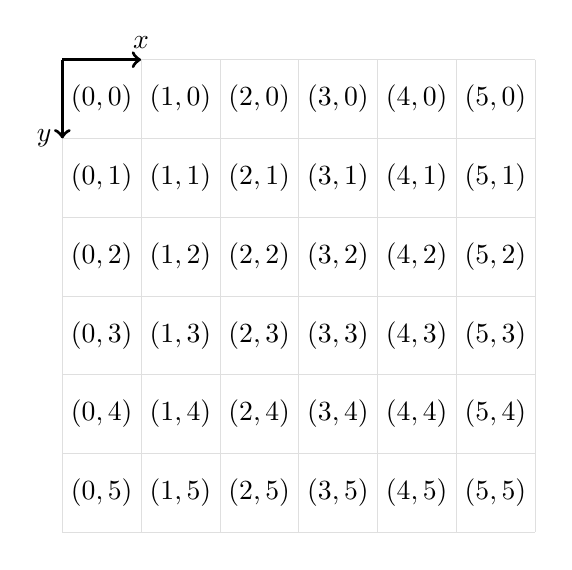
\begin{tikzpicture}[y=-1cm]
        \foreach \i in {\xMin,...,\xMax} {
            \draw [very thin,gray!25] (\i,\yMin) -- (\i,\yMax)  node [below] at (\i,\yMin) {};
        }
        \foreach \i in {\yMin,...,\yMax} {
            \draw [very thin,gray!25] (\xMin,\i) -- (\xMax,\i) node [left] at (\xMin,\i) {};
        }
        \draw[->, very thick] (0,0) -- (1,0) node[above] {$x$};
        \draw[->, very thick] (0,0) -- (0,1) node[left] {$y$};
        \foreach \x in {\xMin,...,5} {
            \foreach \y in {\yMin,...,5} {
                \node at ({\x+0.5},{\y+0.5}) {$(\x, \y)$};
            }
        }
    \end{tikzpicture}
  \end{center}
  \vspace{-20pt}
  \caption{HTML5 canvas plane. Each step is one pixel. There cannot be non-integer
           coordinates.}
  \label{fig:canvas-plane}
  \vspace{-10pt}
\end{wrapfigure}

The data that was used for all experiments was collected with
\href{http://write-math.com}{write-math.com}, a website designed solely for
this purpose. This website makes use of HTML5 canvas elements. Those elements
can be used to track fingers or a mouse coursor touching the canvas, moving
and lifting. The origin is at the upper left corner and get bigger to the right
($x$-coordinate) and to the bottom ($y$-coordinate).

The data is stored and shared in JSON format. Each handdrawing is stored as a
list of lines, where each line consists of tuples $(x, y, t)$, where $x$ and
$y$ are canvas coordinates and $t$ is a timestamp in seconds. This timestamp
gives the time in milliseconds from 1970.

The time resolution between points as well as the resolution of the image
depends on the device that was used. However, most symbols have time resolution
of about $\SI{20}{\milli\second}$ and are within a bounding box of a
$250 \text{px} \times 250 \text{px}$.

\section{Preprocessing}
\subsection{Scaling and shifting}
In many experiments the datapoints were scaled to fit into a unit square while
keeping their aspect ratio. Afterwards, the points were shifted to the
$(0, 1) \times (0, 1)$ unit square. The algorithm is given in pseudocode on
\cpageref{alg:scale-and-shift}. It was shown in \cite{Kirsch,Huang09} that
this kind of preprocessing boosts classification accuracy significantly.

\section{Features}
A number of different features have been suggested so far for on-line handwriting
recognition. They can be grouped into local features and global features.
Local features apply to a given point on the drawing plane and sometimes even
only to point on the drawn curve whereas global features apply to a complete
line or even the complete image.

\subsection{Local features}
\begin{itemize}
    \item Curvature\cite{Manke95}
    \item Speed\cite{Huang09}
    \item Binary pen pressure\cite{Kosmala98,Kosmala11}
    \item Direction\cite{Manke95,Huang06}
    \item Bitmap-environment\cite{Manke95}
\end{itemize}

\cite{Kosmala98,Kosmala11} suggest that speed is a bad feature, because it \enquote{highly inconsistent}.

\subsection{Global features}
\begin{itemize}
    \item Re-curvature\cite{Huang06} (TODO: Explain (all))
    \item Center point\cite{Huang06}
    \item Stroke length\cite{Huang06}
    \item Number of strokes\cite{Huang09}
    \item Pseudo-Zernike Features (TODO: Really global? What is it?)\cite{Khotanzad}
    \item Shadow Code Features\cite{Khotanzad}
\end{itemize}